% \section{Selection of the datasets}\label{app:datasets}

% The deep meta-reinforcement learning framework forces us to define a set of environments associated to image classification tasks. In that regard, we have considered the meta-dataset~\citep{MetaDataset}, which has been used for few-shot learning classification tasks on meta-learning setups. Since the latter is different than the standard classification that we aim for, it is important to define a different sampling strategy than the one originally proposed. Our interest is in choosing small but yet challenging datasets that allow us to save computational resources without making the Neural Architecture Search (NAS) trivial.

% The first step in this process is to discard the datasets that are big in the total number of observations. Ideally, we would like to have smaller datasets than CIFAR-10 (60K observations), which is the reference dataset for NAS. In Table~\ref{tab:appA:metadataset} the complete list of instances in the collection is shown, from which it can be noticed that the only datasets satisfying the criterion are \textit{aircraft}, \textit{cu\_birds}, \textit{dtd}, \textit{omniglot}, \textit{traffic\_sign} and \textit{vgg\_flower}.



% \begin{table}[ht]
% \centering
% \begin{tabular}{cccc}
% \hline
% Dataset ID    & Dataset name                              & N classes & N observations \\ \hline
% aircraft      & FGVC-Aircraft                             & 100       & 10000          \\
% cu\_birds     & CUB-200-2011                              & 200       & 11788          \\
% dtd           & Describable Textures                      & 47        & 5640           \\
% fungi         & FGVCx Fungi                               & 1394      & 89760          \\
% ilsvrc\_2012  & ImageNet                                  & 1000      & 1280764        \\
% mscoco        & Common Objects in Context                 & 80        & 330000         \\
% omniglot      & Omniglot                                  & 1623      & 32460          \\
% quickdraw     & Quick, Draw!                              & 345       & 50426266       \\
% traffic\_sign & German Traffic Sign Recognition Benchmark & 43        & 39209          \\
% vgg\_flower   & VGG Flower                                & 102       & 8189           \\ \hline
% \end{tabular}
% \caption{The original meta-dataset with the number of classes an observations after conversion with the original source code~\citep{MetaDataset}.}
% \label{tab:appA:metadataset}
% \end{table}

% Once the candidate datasets have been selected, we performed a short deep meta-reinforcement learning trial with $t_{max}=200$, default values for all the other parameters of A2C in the OpenAI baselines~\citep{openaibaselines}, $d=10$, $\text{epochs}=12$ and $\text{batch size}=128$. Since at the beginning of the trial the agent is not able to develop any significant knowledge, the network sampling could be seen as a random procedure. In Figure~\ref{fig:appA:trialstats} the boxplot and histogram of the obtained accuracy values are presented, in Figure~\ref{fig:appA:evolution} the evolution of rewards is plotted, and in Table~\ref{tab:appA:times} the running time per experiment is shown. 



% \begin{table}[ht]
% \centering
% \begin{tabular}{cc}
% \hline
% Dataset ID    & Time   \\ \hline
% aircraft      & 9h49m  \\
% cu\_birds     & 16h20m \\
% dtd           & 5h38m  \\
% omniglot      & 3h38m  \\
% traffic\_sign & 4h33m  \\
% vgg\_flower   & 4h56m  \\ \hline
% \end{tabular}
% \caption{Running times of our experiment}
% \label{tab:appA:times}
% \end{table}

% \begin{figure}[ht]
% \centering
% \begin{subfigure}{.5\textwidth}
%   \centering
%       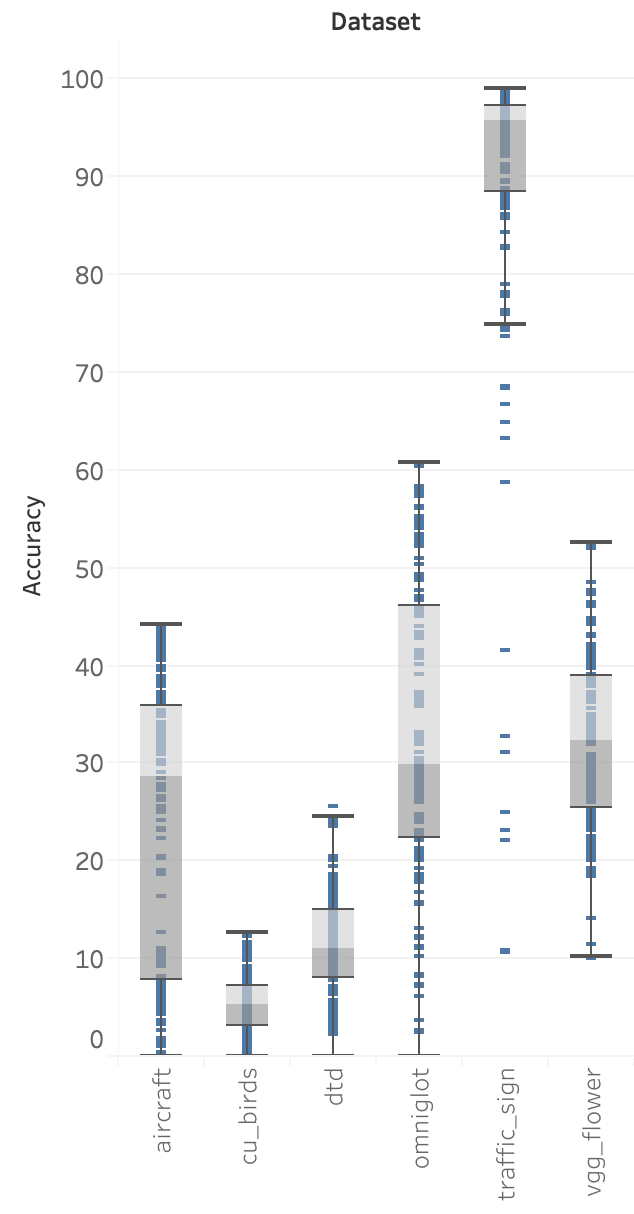
\includegraphics[width=0.8\linewidth]{imgs/boxplot-accuracies.png}
%   \caption{Boxplot of early-stop accuracy values for a subset of the meta-dataset.}
%   \label{fig:appA:boxplot}
% \end{subfigure}%
% \begin{subfigure}{.5\textwidth}
%   \centering
%       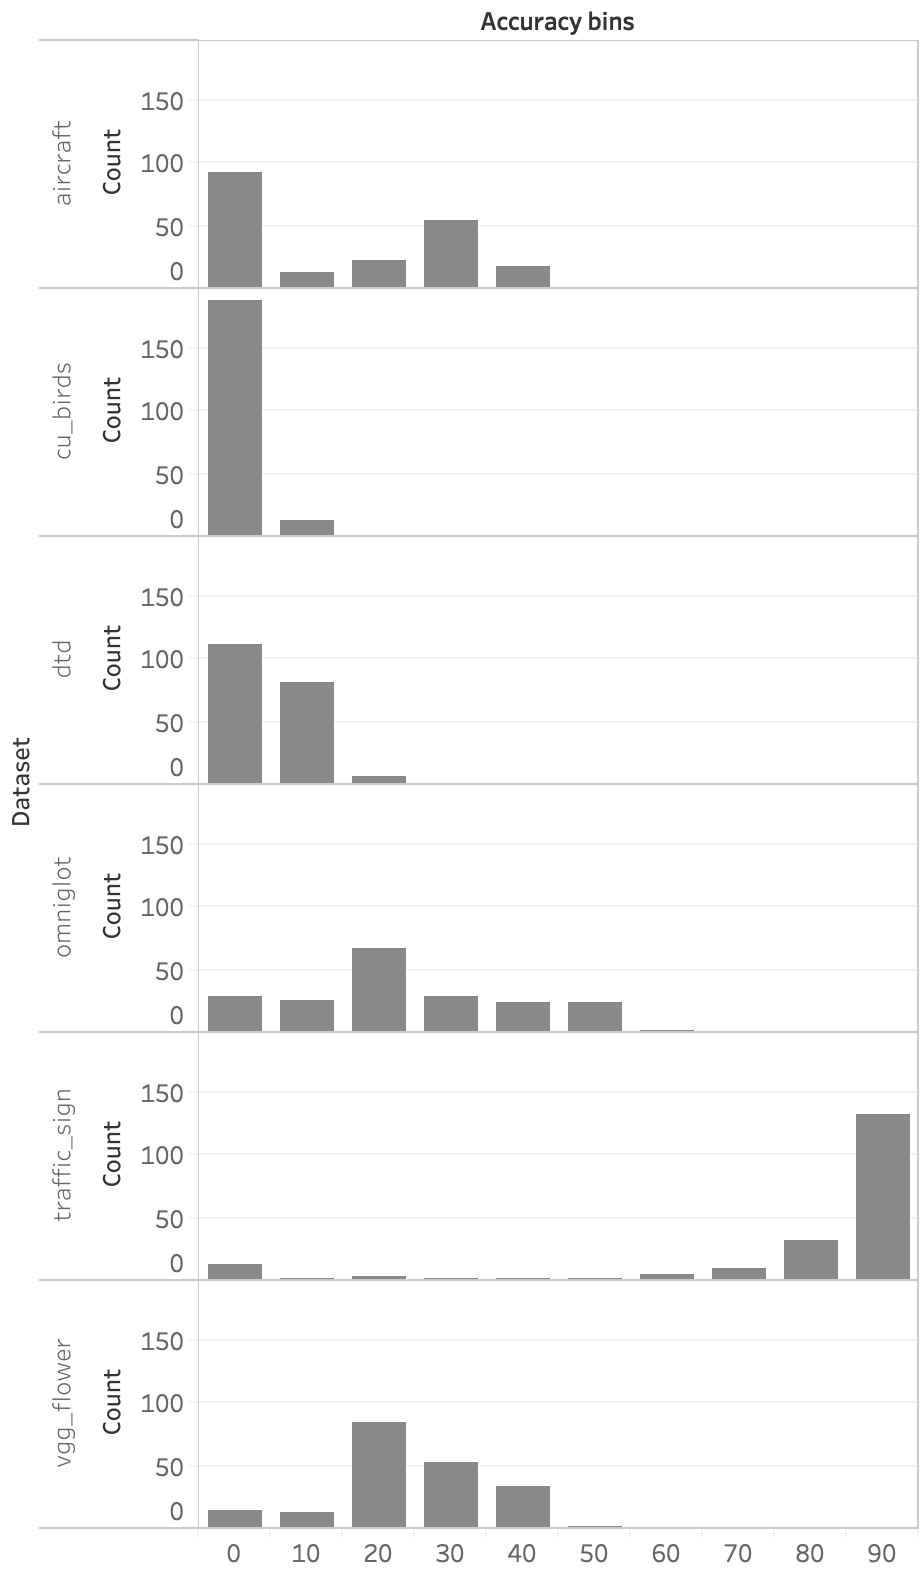
\includegraphics[width=0.9\linewidth]{imgs/histogram-accuracies.png}
%   \caption{Histogram of accuracy values for a subset of the meta-dataset}
%   \label{fig:appA:histogram}
% \end{subfigure}
% \caption{Different visualizations of the early-stop accuracy values obtained in a short deep meta-reinforcement learning trial.}
% \label{fig:appA:trialstats}
% \end{figure}


% \begin{figure}[ht]
%   \centering
%       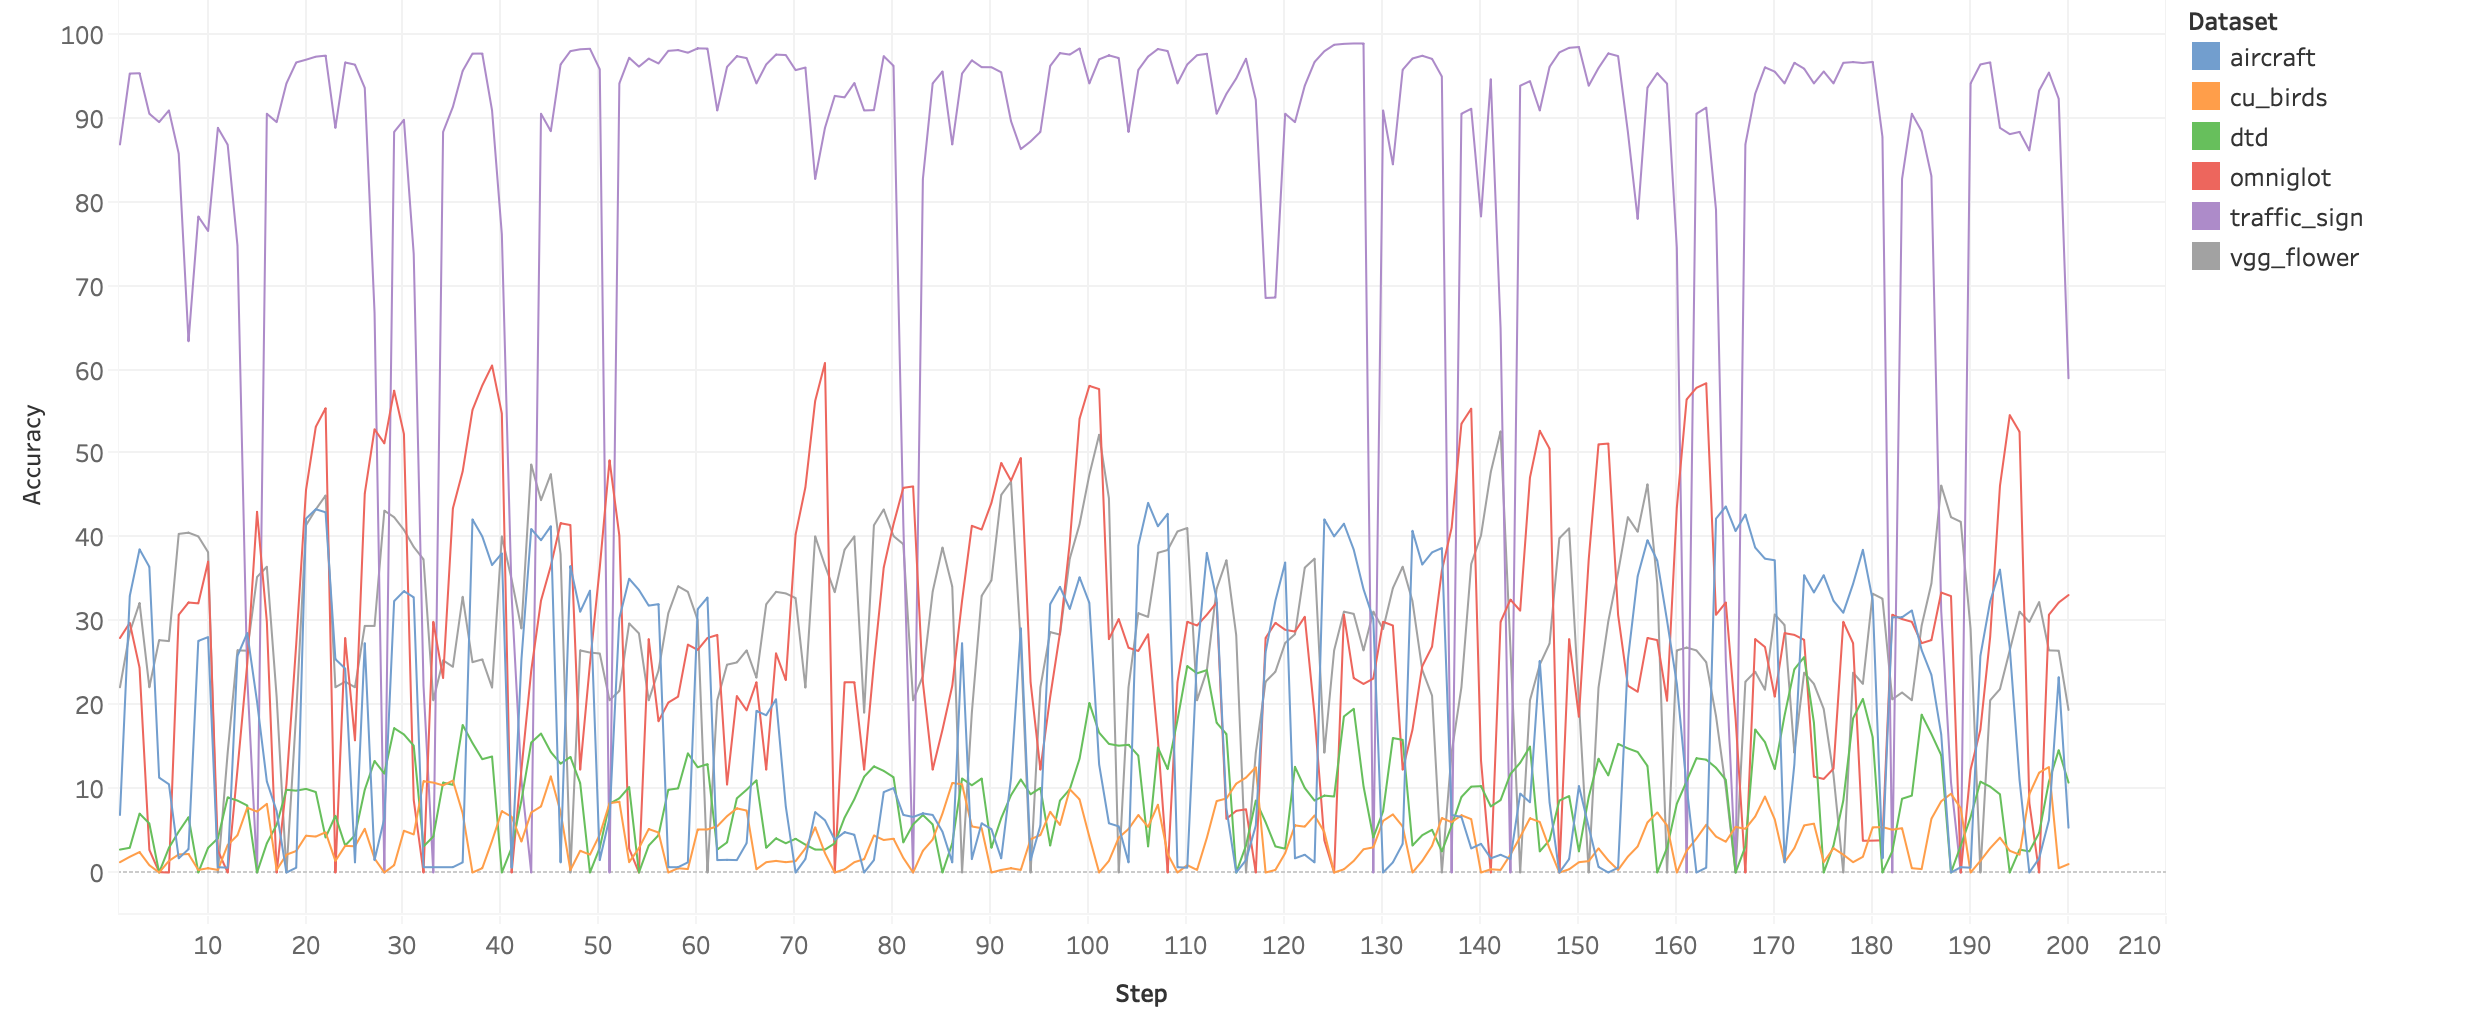
\includegraphics[width=\linewidth]{imgs/all-accuracies.png}
%   \caption{Evolution of early-stop accuracy values for a short deep meta-reinforcement learning trial.}
%   \label{fig:appA:evolution}
% \end{figure}

% This simple exploratory analysis\footnote{A more elaborated analysis would end up in biasing the Neural Architecture Search we aim for, since it would be possible to feed the agent with previous knowledge of the tasks.} suggests three types of datasets: a ``trivial" dataset with high accuracy values with simple networks (\textit{traffic\_sign}), two ``hard" datasets with low accuracy values (all values below 30\%: \textit{dtd} and \textit{cu\_birds}), and three ``medium" datasets with more diversity of accuracy values (median around 30\% and broader interquartile range: \textit{aircraft}, \textit{omniglot}, \textit{vgg\_flower}). On the other hand, for the running times, we can observe that \textit{aircraft} and \textit{cu\_birds} result in expensive experiments, whilst the other 4 are more feasible to complete with our limited computational resources. 

% Considering the computation time, and the hardness of the classification tasks we defined the sampling presented in section~\ref{sec:methodology:rl:environments}, where we have preferred the least-expensive datasets for training.


%%%%%%%%%%%%%%%%%%%%%%%%%%%%%%

\section{Selection of the datasets}\label{app:datasets}

The deep meta-reinforcement learning framework that we implement requires a set of environments associated to image classification tasks. In order to design these environments, we rely on the meta-dataset~\citep{MetaDataset}, a collection of 10 datasets with a concrete sampling procedure designed for meta-learning in few-shot learning image classification. In our setting, the datasets are intended for standard image classification, thus we redefine the sampling strategy. Our interest is in using small but yet challenging datasets that allow us to save computational resources without making the Neural Architecture Search (NAS) trivial.

In Table~\ref{tab:appA:metadataset} the original datasets in the collection are listed. We select the ones that are smaller than CIFAR-10 (60K observations), which is the reference for NAS. The datasets satisfying the criterion are \textit{aircraft}, \textit{cu\_birds}, \textit{dtd}, \textit{omniglot}, \textit{traffic\_sign} and \textit{vgg\_flower}. We want to evaluate the hardness of these six datasets to define a sampling procedure from the collection, and thus we perform a short and individual deep meta-reinforcement learning trial with $t_{max}=200$ for each dataset. Since at the beginning of the trial the agent does not develop any significant knowledge, its sampling of architectures is random. In Figure~\ref{fig:appA:trialstats} the boxplot and barplot of the obtained accuracy values are presented, and in Table~\ref{tab:appA:times} the running time per experiment is shown. 


A simple exploratory analysis suggests three types of datasets: a ``trivial" dataset with high accuracy values with simple networks (\textit{traffic\_sign}), two ``hard" datasets with low accuracy values (all values below 30\%: \textit{dtd} and \textit{cu\_birds}), and three ``medium" datasets with more diversity of accuracy values (median around 30\% and broader interquartile range: \textit{aircraft}, \textit{omniglot}, \textit{vgg\_flower}). On the other hand, for the running times, we can observe that \textit{aircraft} and \textit{cu\_birds} result in the most expensive runs. Considering the computation time, and the hardness of the classification tasks, we defined the sampling presented in Table~\ref{tab:methodology:environments:datasets}. Our training datasets have different levels of hardness and reported the least costly runs.

\begin{table}[ht]
\centering
\begin{tabular}{cccc}
\hline
Dataset ID    & Dataset name                              & N classes & N observations \\ \hline
aircraft      & FGVC-Aircraft                             & 100       & 10000          \\
cu\_birds     & CUB-200-2011                              & 200       & 11788          \\
dtd           & Describable Textures                      & 47        & 5640           \\
fungi         & FGVCx Fungi                               & 1394      & 89760          \\
ilsvrc\_2012  & ImageNet                                  & 1000      & 1280764        \\
mscoco        & Common Objects in Context                 & 80        & 330000         \\
omniglot      & Omniglot                                  & 1623      & 32460          \\
quickdraw     & Quick, Draw!                              & 345       & 50426266       \\
traffic\_sign & German Traffic Sign Recognition Benchmark & 43        & 39209          \\
vgg\_flower   & VGG Flower                                & 102       & 8189           \\ \hline
\end{tabular}
\caption{The original meta-dataset~\citep{MetaDataset} with the number of classes and observations after conversion with the official source code.}
\label{tab:appA:metadataset}
\end{table}



\begin{table}[ht]
\centering
\begin{tabular}{cc}
\hline
Dataset ID    & Time   \\ \hline
aircraft      & 9h49m  \\
cu\_birds     & 16h20m \\
dtd           & 5h38m  \\
omniglot      & 3h38m  \\
traffic\_sign & 4h33m  \\
vgg\_flower   & 4h56m  \\ \hline
\end{tabular}
\caption{Running times of a deep meta-RL trial with $t_{max}=200$, used to study the hardness and cost of each dataset.}
\label{tab:appA:times}
\end{table}

\begin{figure}[ht]
\centering
\begin{subfigure}{.5\textwidth}
  \centering
      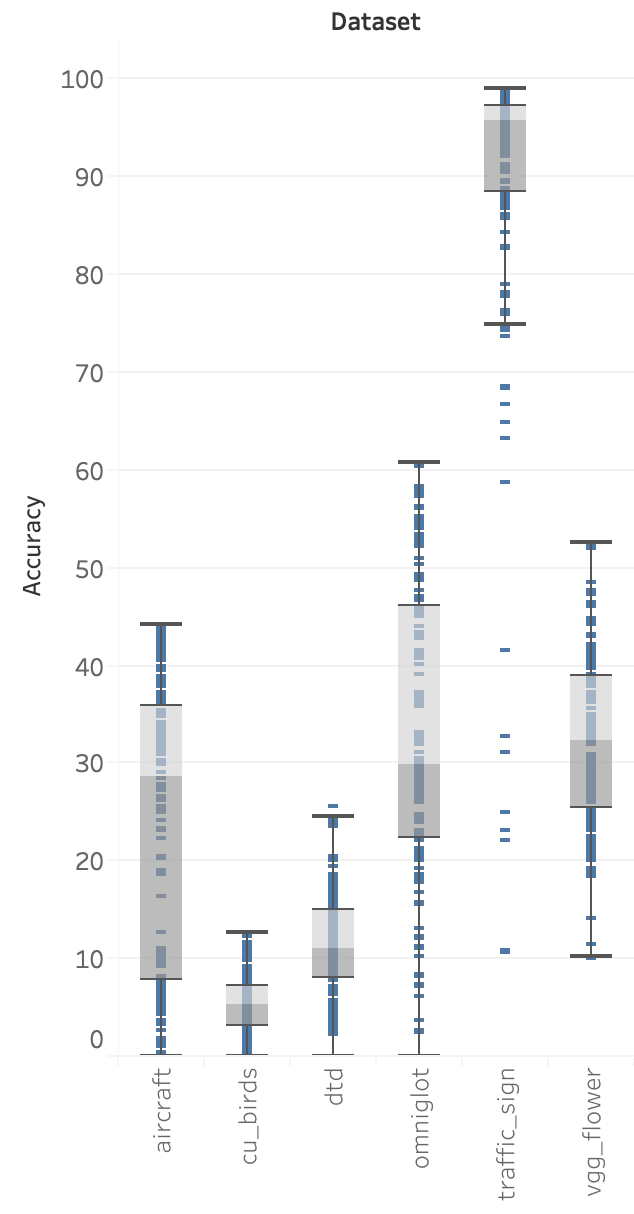
\includegraphics[width=0.8\linewidth]{imgs/boxplot-accuracies.png}
  \caption{}
  \label{fig:appA:boxplot}
\end{subfigure}%
\begin{subfigure}{.5\textwidth}
  \centering
      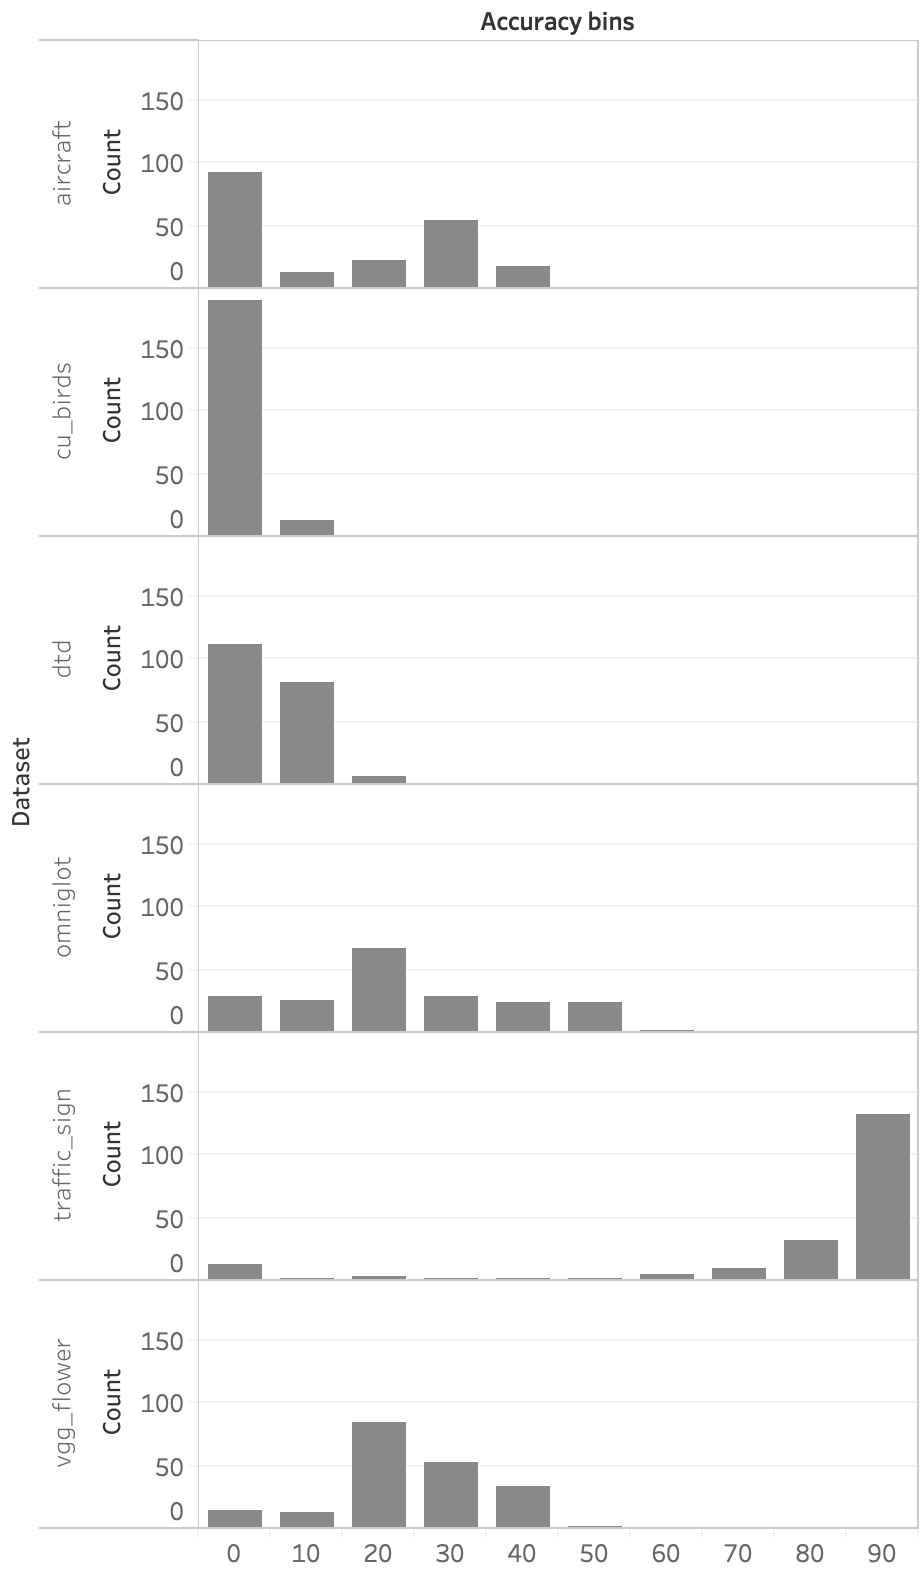
\includegraphics[width=0.9\linewidth]{imgs/histogram-accuracies.png}
  \caption{}
  \label{fig:appA:histogram}
\end{subfigure}
\caption{Different visualizations of the early-stop accuracy values obtained to study the hardness of the datasets.}
\label{fig:appA:trialstats}
\end{figure}


